% !TEX encoding = UTF-8 Unicode
\documentclass[12pt,a4paper,english
% ,twoside,openright
]{tunithesis}

% Note that you must choose either Finnish or English here and there in this
% file.
% Other options for document class
  % ,twoside,openright   % If printing on both sides (>80 pages)
  % ,twocolumn           % Can be used in lab reports, not in theses

% Ensure the correct Pdf size (not needed in all environments)
\special{papersize=210mm,297mm}


% LaTeX file for BSC/MSc theses and lab reports.
% Requires the class file (=template) tunithesis.cls and figure files,
% either tut-logo, exampleFig (as pdf or eps) and example_code.c
% Author: Lucas Machado (2018)
% Based on TTU template by Sami Paavilainen (2006), modified by Heikki Huttunen (2014)


% More information about Latex basics:
% [Tobias Oetiker, Hubert Partl, Irene Hyna, Elisabeth Schlegl, The
% Not So Short Introduction to LATEX2e, Version 5.03, April 2014, 171
% pages.  Availbale: http://tobi.oetiker.ch/lshort/lshort.pdf]


%
% Define your basic information
%
\author{Forename Surname}
\title{Thesis title} % primary title (for front page)
\thesistype{Master's thesis} % or Bachelor of Science, Laboratory Report... 

% Put your thesis' main language last
% http://mirrors.ctan.org/macros/latex/required/babel/base/babel.pdf
\usepackage{lastpage}
\usepackage[english]{babel}
\usepackage[
backend=biber,
style=authoryear,
citestyle=authoryear,
autocite=inline
]{biblatex}
\usepackage{csquotes}

\addbibresource{thesis_refs.bib} %Imports bibliography file

%
% You can include special packages or define new commands here at the
% beginning. Options are given in brackets and package name is in
% braces:  \usepackage{opt]{pkg_name}

% Option1) for bibliography does not need additional packages.

% Option2b) for bibliography: old way for using Name-year citations
% http://www.ctan.org/tex-archive/macros/latex/contrib/harvard/ 
%\usepackage{harvard}  


% Option3) for bibliography: newer way, esp. for Name-year citations
% http://www.ctan.org/pkg/biblatex
%\usepackage[style=authoryear,maxcitenames=2,backend=bibtex,
%  firstinits=true]{biblatex}
%% Note that option style=numeric works as well
%\addbibresource{thesis_refs.bib}

\definecolor{tunipurple}{RGB}{78, 0, 142}

% You can also add your own commands
\newcommand\todo[1]{{\color{red}!!!TODO: #1}} % Remark text in braces appears in red
\newcommand{\angs}{\textsl{\AA}}              % , e.g. slanted symbol for Ångstöm

% Preparatory content ends here



\pagenumbering{roman} % was: {Roman}
\pagestyle{headings}
\begin{document}



% Special trick so that internal macros (denoted with @ in their name)
% can be used outside the cls file (e.g. \@author)
\makeatletter



%
% Create the title page.
% First the logo. Check its language.
\thispagestyle{empty}
\vspace*{-.5cm}\noindent

\begin{figure}
    \vspace{-1.3cm}
    \advance\leftskip-2.5cm
    \noindent
\includegraphics{img/tunilogo.png}
\end{figure}
 
\vspace{2.5cm}
\begin{flushright}
\noindent\textsf{\LARGE{\@author}}

\noindent\vspace{0.5cm}

\noindent\Huge{\textsf{\textbf{\textcolor{tunipurple}{\@title}}}}
\end{flushright}
\vspace{13.7cm} % adjust to 12.7 this if thesis title needs two lines

% Last some additional info to the bottom-right corner
\begin{flushright}  
    \begin{spacing}{1.0}
      \textsf{Faculty of Information Technology and Communication Sciences (ITC)\\
      \@thesistype\\
      April 2019}
    \end{spacing}
\end{flushright}

% Leave the backside of title page empty in twoside mode
\if@twoside
\clearpage
\fi

% Turn off page numbering for the first pages
\pagenumbering{gobble}


% Some fields in abstract are automated, namely those with \@ (author,
% title, thesis type).

\chapter*{Abstract}

\begin{spacing}{1.0}
\noindent \@author: \@title\\
\@thesistype\\
Tampere University\\
Master’s Degree Programme in Software Development\\
April 2019
\end{spacing}
\noindent\rule{12cm}{0.4pt}

\vspace{0.5cm}

% ---------------------------------------
% Abstract and keywords
% ---------------------------------------

\noindent The abstract is a concise 1-page description of the work: what was the
problem, what was done, and what are the results. Do not include
charts or tables in the abstract.

These instructions are intended for students of Computer Sciences at the Tampere University. They cover questions of writing a thesis, such as use of the literature, structure of the thesis and style, the external appearance of the thesis and the use of tools.  These instructions do not cover the scientific content of the thesis.

~

\noindent\textbf{Keywords:} M.Sc. thesis, layout, writing style.

~

\noindent The originality of this thesis has been checked using the Turnitin Originality Check service.


% Add the table of contents


\setcounter{tocdepth}{3}              % How many header level are included
\tableofcontents                      % Create TOC


% The actual text begins here and page numbering changes to 1,2...
% Leave the backside of title empty in twoside mode
\if@twoside
%\newpage
\cleardoublepage
\fi


\renewcommand{\chaptername}{} % This disables the prefix 'Chapter' or
                              % 'Luku' in page headers (in 'twoside'
                              % mode)


\chapter{Introduction}
\label{ch:intro} 

\pagenumbering{arabic}
\setcounter{page}{1} % Start numbering from zero because command
                     % 'chapter*' does page break
                     
% \label{...} allows cross-referencing, e.g. 'as explained in
% Chapter~\ref{ch:intro}' Note that you may have to run the command
% 'latex' or 'pdflatex' twice to get cross-references correctly.  You
% can add labels e.g. to chapters, sections, figures, tables, and
% equations.

% You can write everything into single tex file. Alternatively, you
% can write each chapter into separate file and then include them her
% \include{intro} % no postfix .tex to the command
% \include{related_works} % and so on...


These instructions concern the writing of the Master’s thesis (in Finnish pro gradu ‑tutkielma) to be referred to hereafter as ‘thesis’.  They can also be applied to the writing of other types of academic texts.  The general instructions regarding theses appear in the Opinto-opas (study guide).  The purpose of the present text is to provide some practical advice and describe practices adhered to in the School of InformationDegree Program of Computer Sciences.  The instructions are in no way absolutely binding, but departing from them should be done with consideration.  Practices may differ between supervisors, thus it is always advisable to consult the supervisor on these issues.

These instructions do not cover research methods or matters pertaining to the content of the thesis.

Introduction outlines the purpose and objectives of the presented
research. The background information, utilized methods and source
material are presented next at a level that is necessary to understand
the rest of the text. Then comes the discussion regarding the achieved
results, their significance, error sources, deviations from the
expected results, and the reliability of your research. Conclusions is
the most important chapter. It does repeat the details already
presented, but summarizes and them and analyzes their
consequences. List of references enables your reader to find the cited
sources.


This document is structured as follows. Chapter~\ref{ch:style}
discusses briefly the basics of writing and presentation style
regarding the text, figures, tables and mathematical
notations. Chapters~\ref{sec:ref_styles} and \ref{ch:concl} summarize
the referencing basics and the whole document. There are two example
appendices as well (Appendix A and B).
% ~\ref{app:A} and \ref{app:B}). Labels do not with \chapter*


\chapter{Writing style}
\label{ch:style}

Effective written communication requires both sound content and clear
style. Keep the layout of your thesis neat and pay attention to your
writing style.

\section{Using LaTeX}

This document serves as an example, rather than tutorial, since there
are plenty of those available, see for example 
\cite{mittelbach04,oetiker14, latex13}. The source files are compiled
with the command \texttt{pdflatex d\_tyo.tex} (or \texttt{latex
  d\_tyo.tex}). Depending on your bibliography style, you might also
need to run \texttt{bibtex d\_tyo}.

Unfortunately, compilation may fail, if your LaTeX environment does
not have all the needed packages installed. If you cannot install
them, you can momentarily disable them by putting them inside comments
in the file tutthesis.cls:
\begin{center}
\texttt{\% \textbackslash usepackage\{hyperref\}}
\end{center}
Of course, depending on the package, some of the features are also
disabled and you must remove those parts from your tex file.
Spellchecking can done, for example, by running 
\texttt{aspell -t -c d\_tyo.tex}.

Moreover, certain characters need escape symbols, e.g. per cent should
be written as \textbackslash\% (otherwise it starts a comment),
underscore as \textbackslash\_, tilde as \textbackslash\~{}\{\}, hash
as \textbackslash\#, dollar sign as \textbackslash\$, and opening
brace as \textbackslash\{ and so on. Note that double backslash
\textbackslash\textbackslash makes a line break.

\section{Text}
A thesis is written with a single-column layout on one- or two-sided
A4 sheets (210 mm x 297 mm). The font type of the body text is usually
Times New Roman and the font size is 12 pt. The spacing is 1.2 and the
text is fully justified and hyphenated. You do not have to indent the
paragraphs.

Arial 18 pt font is used for the headings in this guide, and there is
a 42 pt space above and below. The font size of subheadings is
14. There is an18 pt space above subheadings and 12 pt space below
them.

Brief basics of writing style are:
\begin{itemize}
\item Always think of your reader when you are writing and proceed
  logically from general to specific.
\item Highlight your key points, for example, by discussing them in
  separate chapters or presenting them in a table or figure. Use
  \textit{italics} or \textbf{boldface} for emphasis, but don't overdo
  it.  Moreover, this template uses \texttt{teletype} font for LaTeX
  specific names, such as commands and files.
\item Avoid long sentences and complicated statements. A full stop is
  the best way to end a sentence.
\item Use active verbs to make a dynamic impression but avoid the
  first person pro-noun ``I'', except in your preface.
\item Avoid jargon and wordiness. Use established terminology and
  neutral language.
\item The minimum length of chapters and subchapters is two
  paragraphs, and you need to consider the balance of
  chapters. Paragraphs must always consist of more than one sentence.
\item Do not use more than three levels of headings, such as 4.4.2.
\item Do not use too many abbreviations. Use capital and small letter
  consistently
\end{itemize}

Sometimes ending a section with list is considered as bad
style. Therefore, it is better to have some text after it.


\section{Figures}
You must refer to all the figures in the body text. The reference
should preferably appear on the same page as the actual figure or
before it. Figures and tables must be numbered consistently thesis
and primarily placed at the top of the page, but you are free to
decide where they fit best. Never start a chapter with a figure, table
or list.

Figures and the caption are either consistently centered (or aligned
to the left). The caption is placed under the figure and always on the
same page as the figure. All figures must be explained in the body
text, so that readers know what they are supposed to notice. Figures
generated by analysis software usually need further editing, see
Figure~\ref{fig:ex_fig} for example. The figures should be in the same
language as other text (even if Figure~\ref{fig:ex_fig} violates this
recommendation). The recommended font size is the same as that of the
body text but no smaller than 10 pt. The figures must be readable,
even if your thesis is printed in greyscale.
% Note: put tilde between text and ref command, like in
% 'Figure~\ref{fig:ex_fig}' above. Tilde (~) puts a white space but
% prevents line break. Same thing applies to Table~\ref{tab:summary}
% as well.

% Here's an example how to add a figure. Default placement of figures
% is at top of page, i.e. placement specifier is '[t]' could be
% omitted.  The dimensions can be relative to text width (or height)
% or absolute (4 cm).

% You can leave out the figure postfix (.pdf, .eps, .png). Utilized
% tool (pdflatex, latex...) decides what file type to look for.
% http://en.wikibooks.org/wiki/LaTeX/Importing_Graphics#Compiling_with_latex

% Note that figure is placed _after_ this point and also after the
% previous figures. You can cut-paste the figure insertion point
% earlier to get it in better place, i.e. the figure can be before
% reference to it in the Tex file, but otherway round in final pdf.
% More information: [Oetker, pp. 49-52]. 
\begin{figure}[t]
  \begin{center}
    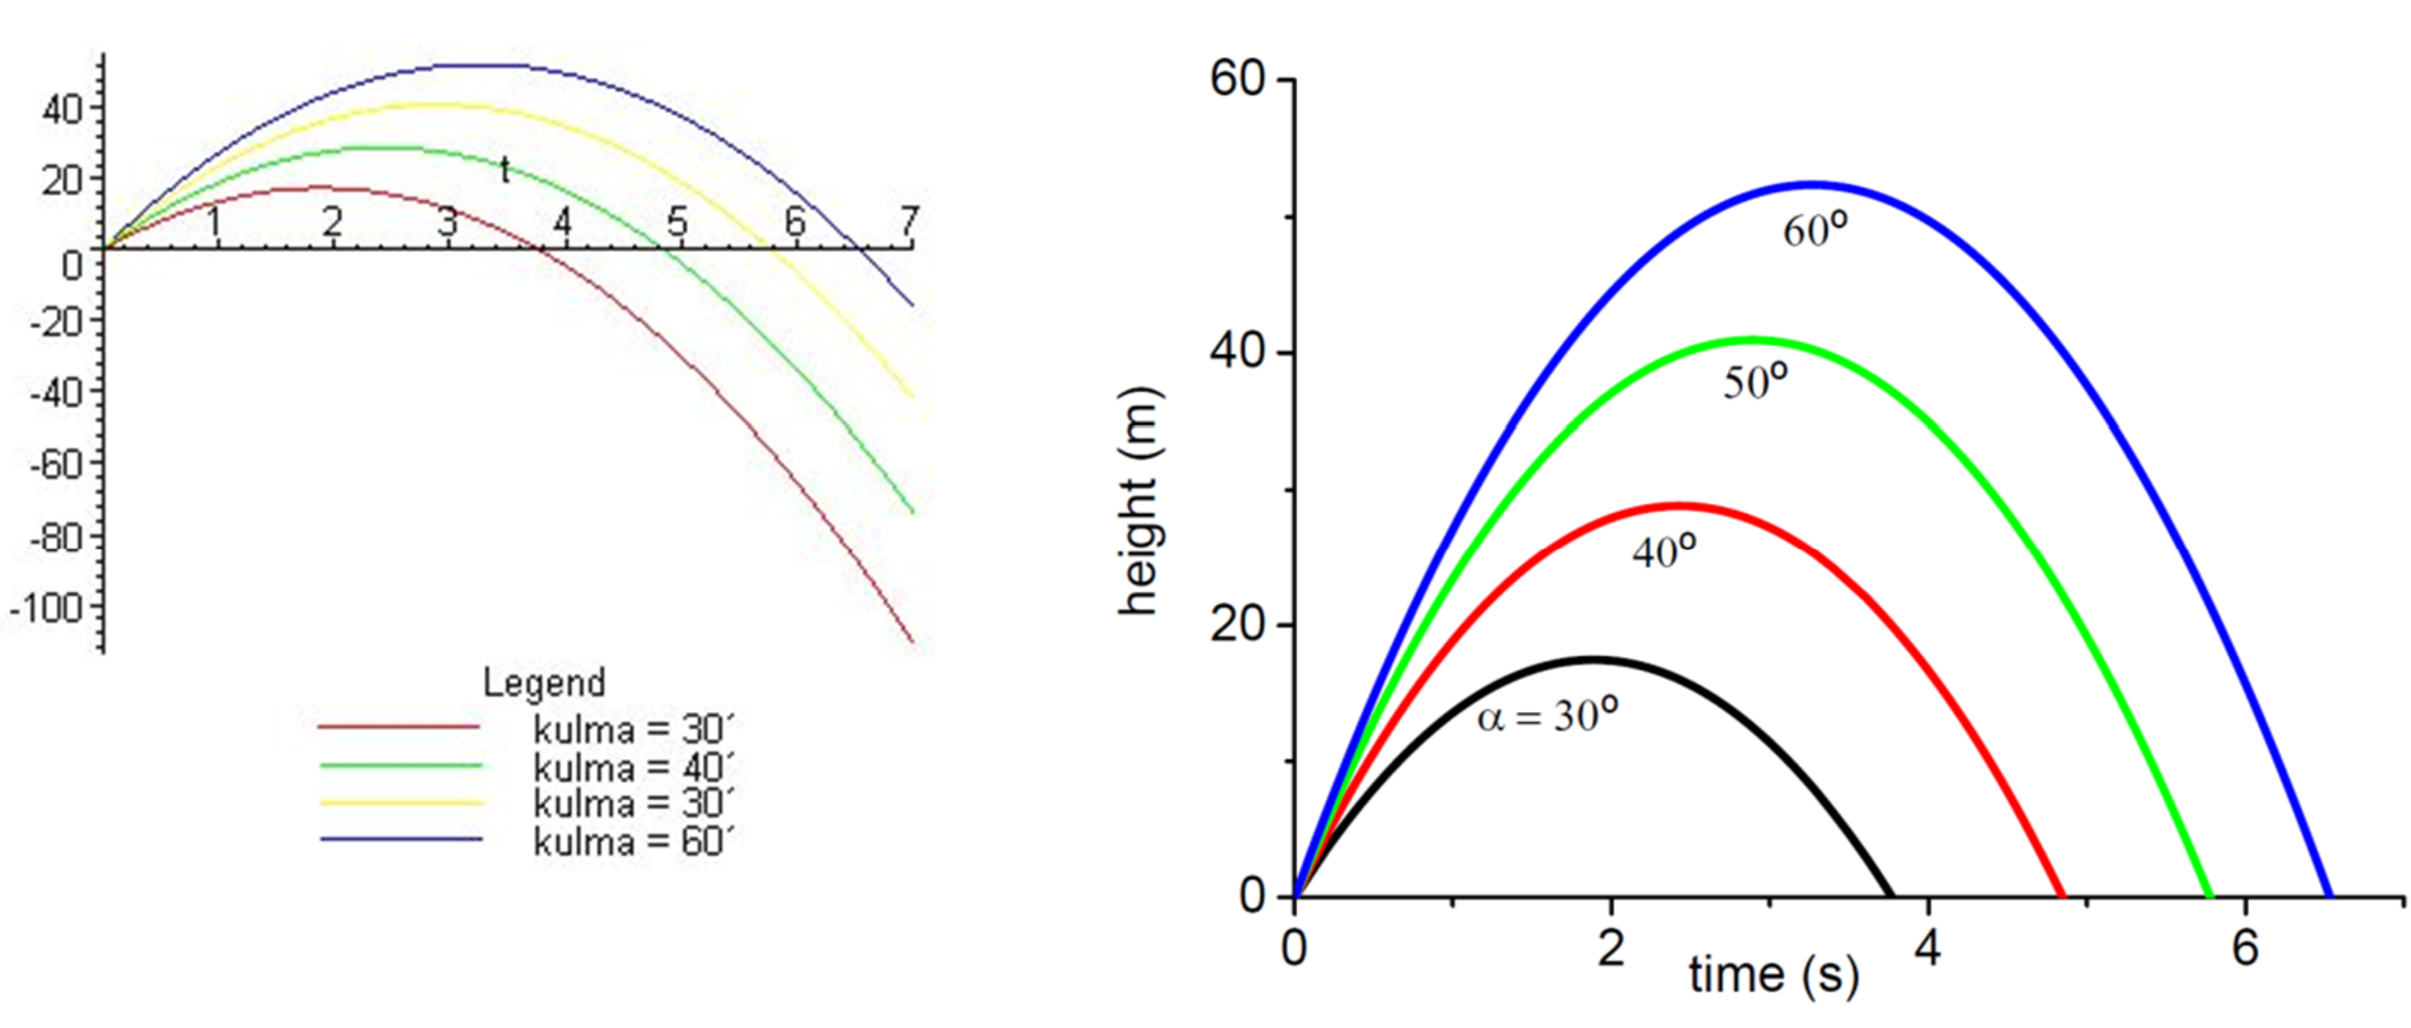
\includegraphics[width=1.0\textwidth]{exampleFig}
  \end{center}
  \caption[Diagrams should be edited before publication.]{Diagrams
    should be edited before publication. The diagram on the right is
    an edited version of the one on the left.}
  % Optional shorter caption in brackets is used in Table of Figures
  % (tof).
  \label{fig:ex_fig}
\end{figure}

% In conference and journals articles with two columns, the
% command \begin{figure*} is useful. The asterisk makes the figure
% width equal to the whole page. The same applies to \begin{table*} as
% well.



The basic command \texttt{latex} accepts only encapsulated postscript
(eps) format. Therefore it is usually easiest to compile with
\texttt{pdflatex} which can handle \verb+*.png+, \verb+*.jpg+ and
\verb+*.pdf+ formats. Eps and pdf are recommended since their support
vector graphics (zooming). For example Figure~\ref{fig:ex_fig} is in
pdf format. 
%Some programs, such as PowerPoint, store pdf figures A4
%sized. Fortunately, pdf editors, such as PDF-X-Change, have a feature
%'remove white spaces' or 'crop'.


LaTeX has a package \texttt{subfigure} to layout multiple figures
together, for example Figure~\ref{subfig:draft} to
\ref{subfig:small_fig}. There might be newer packages as well, but this is
already a quantum leap ahead of some other, unnamed word processors.
% See http://www.ctan.org/pkg/subfigure
\begin{figure*}
  \begin{center}
    \subfigure[Option \texttt{draft} helps to makes a placeholder box for figure. The file must exist.]{
      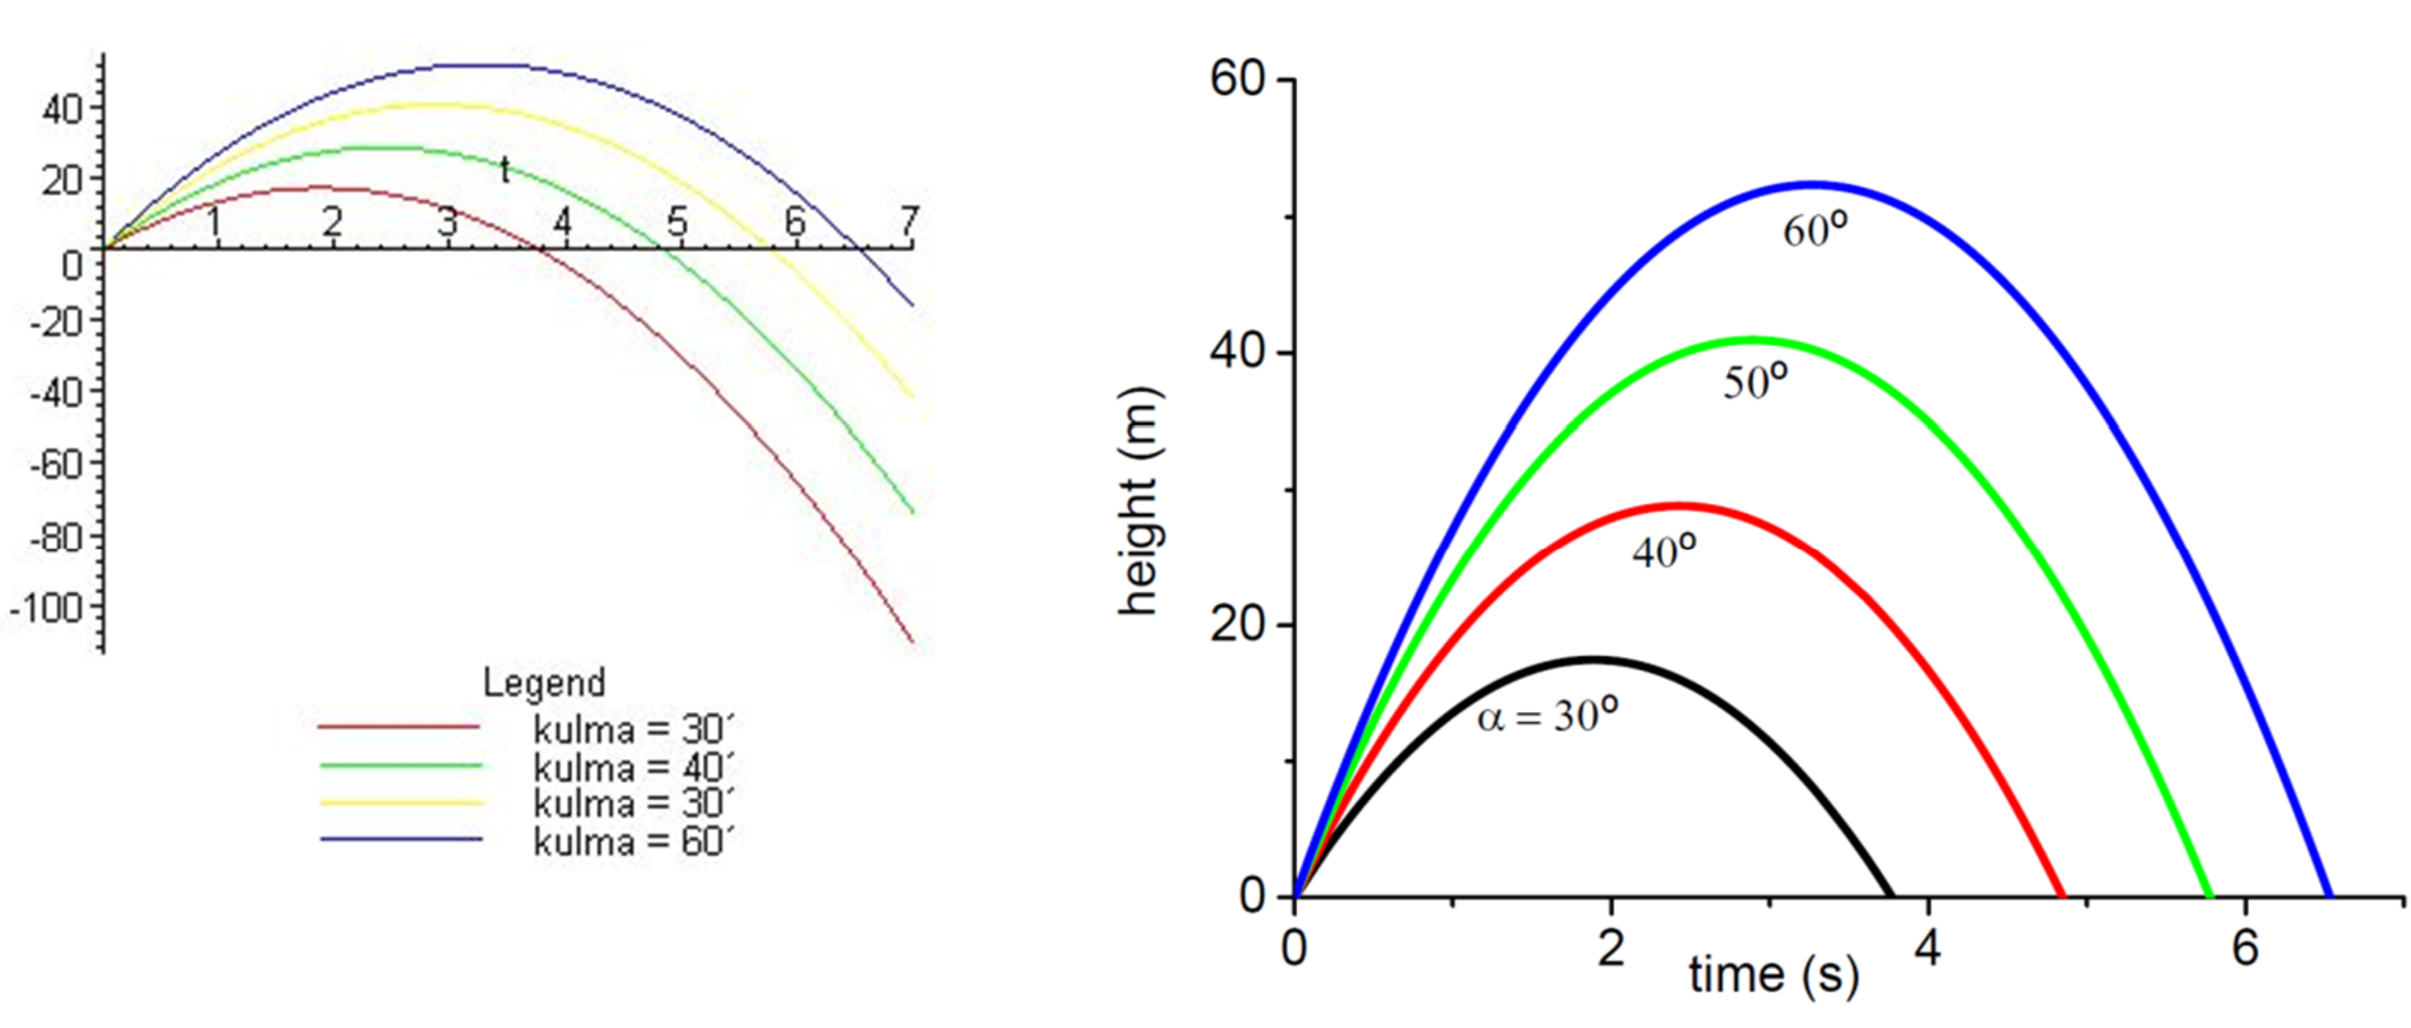
\includegraphics[draft, width=0.35\textwidth]{exampleFig}
      \label{subfig:draft}}
    \qquad                        % i) Ugly hack to get more horizontal space between figures
    %\hspace{0.05\textwidth}      % ii) Another ugly way to hack space
    % ~~                          % iii) Yet another... 
    \subfigure[Another way ot make a placeholder box with the command
      \texttt{rule}.]{
      \textcolor{blue}{\rule{0.3\textwidth}{3cm}}
      \label{subfig:rule}}
    \subfigure[Actual figure included but scaled down.]{
      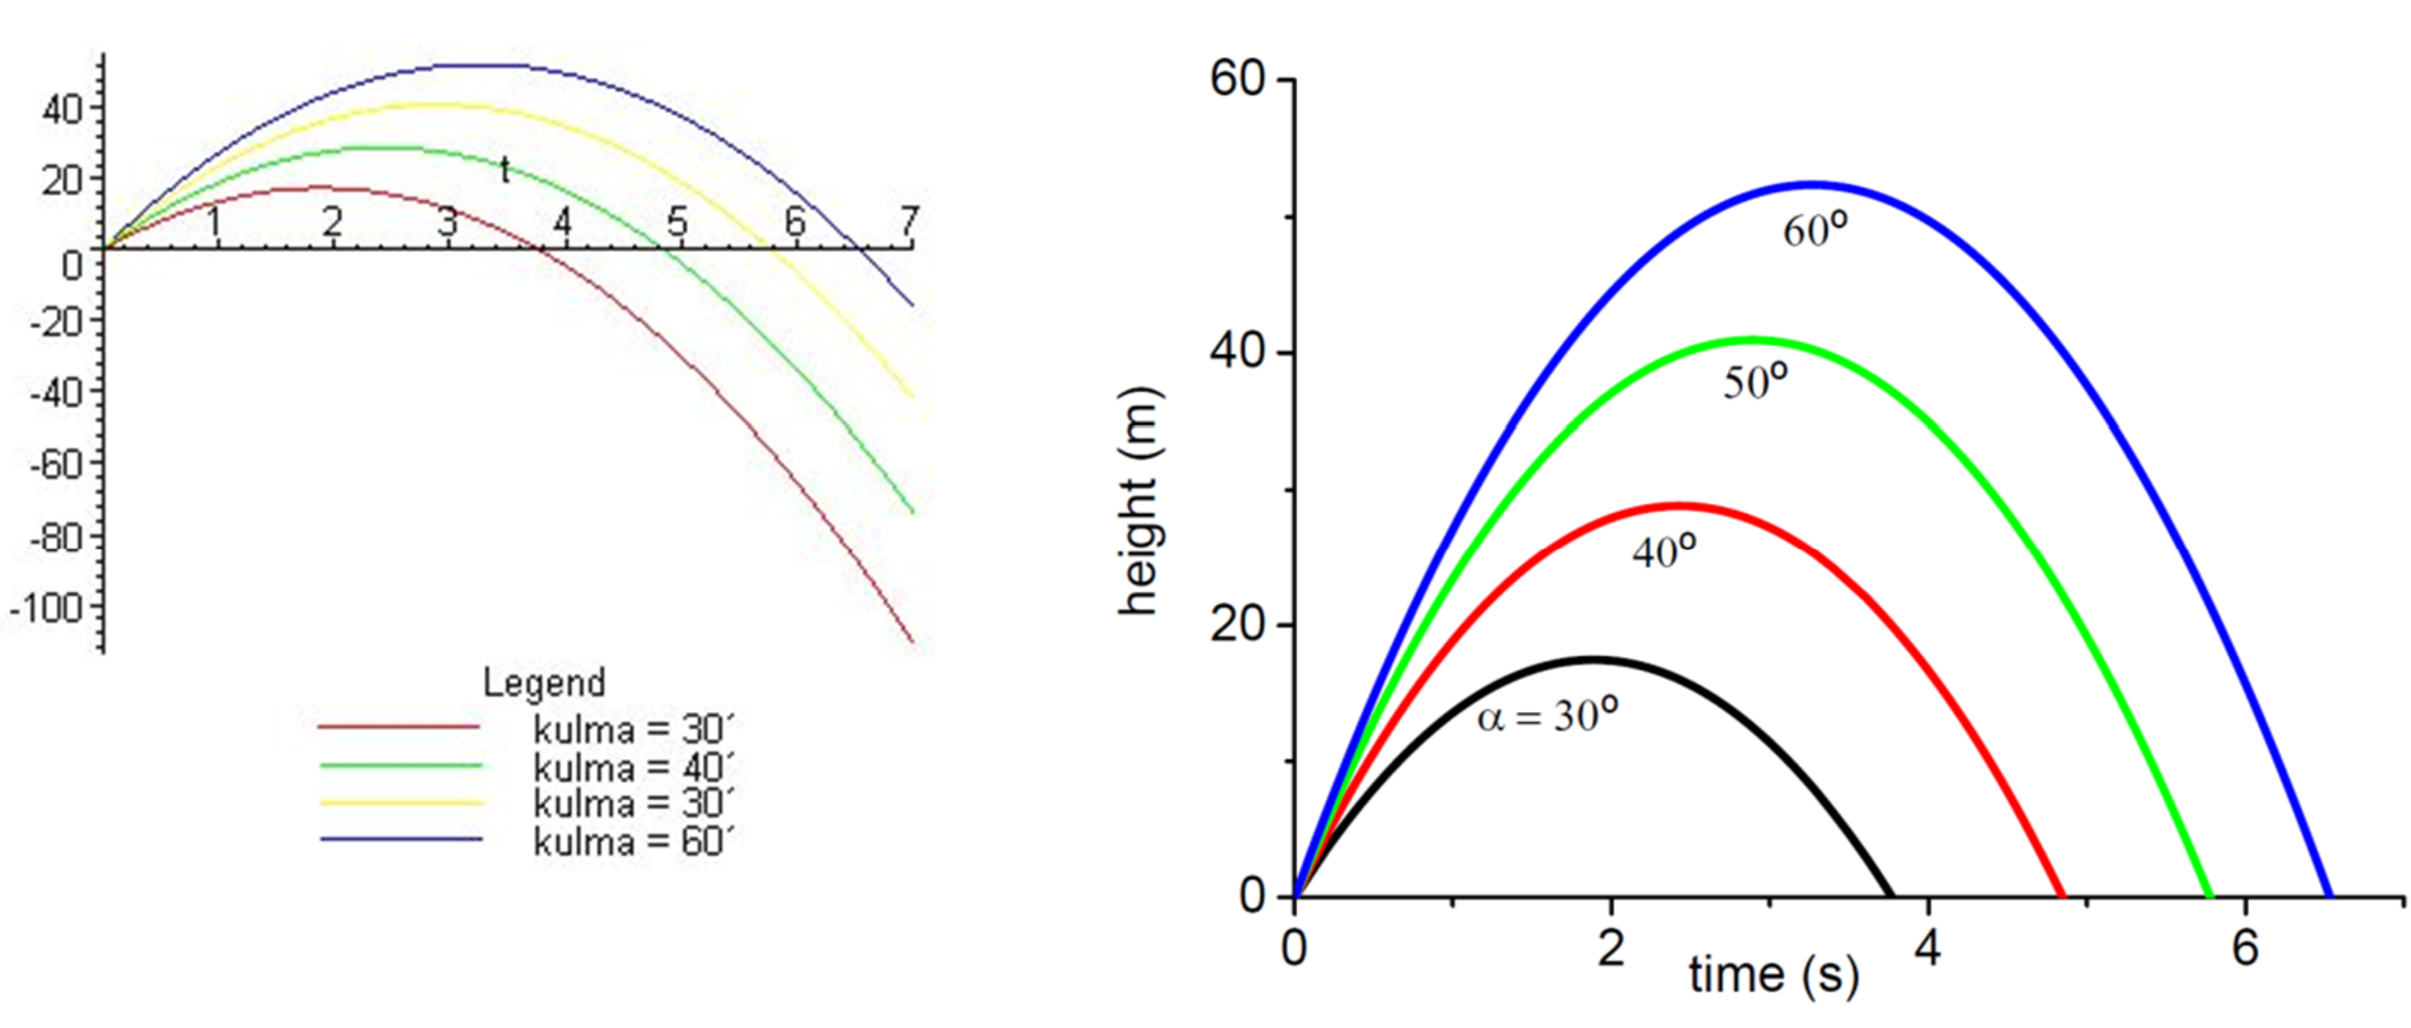
\includegraphics[width=0.35\textwidth]{exampleFig}
      \label{subfig:small_fig}}
    \caption[Example of subfigures]{Example of subfigures. Pay attention to how nicely they
      are laid out and their neat subcaptions.}
    % Optional shorter caption in brackets is used in Table of Figures
    % (tof).

    \label{fig:subfigs}
  \end{center}
\end{figure*}


\section{Tables}

Tables have numbered captions, see Table\ref{tab:thin_film} for
example. The caption is placed on the same page but above the table,
unlike the captions that accompany figures. You must refer to all the
tables in the body text. In addition, you must discuss the content of
any tables in the body text to ensure that readers understand their
relevance.
%
%TODO: translate the thin film explanation in English
%

\todo{translate the thin film explanation in English}

\begin{table}[ht]
  \small
  \begin{center}
    \caption{Example of evaporation conditions in a thin film structure.}
    \label{tab:thin_film}
    \begin{tabular}{l | r r r r r r}
      % l = align to left (e.g. text), c=align to center, r=align to
      % right (e.g. numbers), Pipe | creates vertical line
      % Let's put 1 horinzontal line above the table, 2 after header rows,  and 1 below
      \hline
      \textbf{Substance} & \textbf{Thickness}& \textbf{Correction } & \textbf{Pressure} & \textbf{Temper-}          & \textbf{Current} & \textbf{Speed} \\
                         & \textbf{(nm)}     & \textbf{coefficient} & \textbf{(mbar)}   & \textbf{ature ($^\circ$C)} & \textbf{(mA)}    & \textbf{(nm/s)} \\
      \hline 
      \hline
      SiO2	& 181.0	& 1.10	& $3.0\cdot10^5$	& 90.6	& 20-23	 &0.2 \\
      TiO2	& 122.1	& 1.55	& $1.5\cdot10^4$	& 91.1	& 100-93 &0.1 \\
      \hline
    \end{tabular}
  \end{center}
\end{table}


Often it is better to create the table in, e.g. MS Excel, and import
it as .eps or .pdf file, for example, when you calculate some of the
values automatically.
%\begin{table}[h]
%  \begin{center}
%    \caption{Example of evaporation conditions in a thin film structure.}
%    \label{tab:thin_film_graphics}
%    \includegraphics[width=8cm]{my_table.eps}
%  \end{center}
%\end{table}



The titles of the columns in your table are specified and data is
added to the table. You can use boldface to highlight the titles and
use a double horizontal line to separate the from the rest of the
table. The order of the columns and rows must be carefully
considered. Do not surround all the cells with a border, as it may
make your table harder to read. Put a line on top and bottom of the
table. You can add a horizontal line between every $4-5$ rows, if the
data is not grouped into categories. If the table is large, the rows
should be numbered if you plan to refer to the rows in the body text.

The numbers are right aligned (optimally lined up at the decimal
point) for easy comparison. You should preferably use SI units,
established prefixes and rewrite large numbers so that the power of
ten should be placed in the title of the column instead of each row,
if possible. More suggestions can be found in \cite{salminen09}.

\section{Mathematical notations}

Numbers are generally written using numerals for the sake of clarity,
for example ``6 stages'' rather than ``six stages'', which is
nevertheless strongly preferred to ``a couple of stages''. You should
also use a thousand separators\footnote{Use tilde \~{} in LaTeX and a
  special character \textit{non-breaking space} in MS Word},
i.e. instead of 55700125 write 55~700~125. Never omit the leading zero
in decimals. For example, it is correct to write ``0.5'' and wrong to
write ``.5''. A comma is used as a decimal separator in the Finnish
language and a period in the English language.

Like numbers, it is advisable to abbreviate units of
measurement. There is a space between the number and the unit, but you
should keep them on the same line. It is better to compile a table or
graph than include a great deal of numerical values in the body
text. Use precise language and put numbers on a scale (small, fast,
expensive).

Use generally known and well defined concepts and standard conventions
and symbols for representing them. New concepts should be defined when
they appear in the text for the first time. Upper case and lower case
letters mean different things in symbols and units of measurement. Do
not use the same symbol to mean different things.

Newton's Second Law can be presented in the following way:

\begin{equation}
  \label{eq:newton2}
 ma= F,
\end{equation}

where $m$ denotes the mass of an object, $a$ means acceleration, and
$F$ means force. Please note that all the variables must be defined at
the point of their first appearance. All sen-tences end with a
punctuation mark, and the main elements of a sentence are separated by
a comma in accordance with the rules of English grammar.  Mathematical
formulas are numbered, if they are written on separate lines and
referred to in the main body of the text. The number is usually put in
parenthesis and right aligned, see equation \ref{eq:newton2} for
example. Occasionally mathematical notations are preceded by an
identifier, such as 'Definition 1' or 'Theorem 1'
\cite{ruohonen09}. Simple formulas may be displayed within the body of
the text without numbering.

Do not start a sentence with a mathematical symbol but add some word,
such as the name or type of the symbol, in front of it. Variables,
such as x and y, are generally presented in italics, whereas
elementary functions, special functions and operators are not:
\begin{center}
sin$(2x+y)$, 	grad $T$, 	div $B$, 	lim $(x^2 - 1)/(x + 1)$.
\end{center}

At first, it is better to rely on the automated formatting of an
equation editor. You may have to make compromises between logical
clarity and readability.


LaTeX is the best editor for writing also the more complex equations, such as
\begin{equation}
  \label{eq:fourier}
  G^+(t,t')= \int G^+(E) exp[-iE(t-t')/\hbar] dE.
\end{equation}




\section{Programs and algorithms}

Codes and algorithms are written using monospaced font, such as
Courier New, Consolas or their variations. If the length of the code
or algorithm is less than 10 lines and you do not refer to it later on
in the text, you can present it similarly to formulas.  Here's an
example showing a snippet from the makefile. These commands were
written directly to the .tex file and appear without numbering.

\begin{lstlisting}[style=console, % title={Template files}
  ] 
all: ${TARGET}.tex
	pdflatex ${TARGET}.tex
	bibtex ${TARGET}
	pdflatex ${TARGET}.tex
\end{lstlisting}  
% You can add an extra dollar sign here to turn off the accidental
% syntax highlight (when there is an odd number of dollar signs in
% listing)

If the code is longer but shorter than a page, you present like a
figure (Program 4.1) titled ``Program'' or ``Algorithm''.
% This is controlled from .cls file with command
% \renewcommand\lstlistingname{Program} % or {Ohjelma} in Finnish
You should add some comments to the code and indent it
consistently. The actions performed by the code must be outlined in
broad terms in the body text. Line numbers make it much easier to
refer to the code in the text. 

LaTeX has a package listings \cite{heinz06} which can handle code
very conveniently, include real code files, add row numbers, and
highlight the reserved words.  Program~\ref{code:sort} shows another
example which is included from a separate file
\textit{example\_code.c}, and includes both line numbers and a code
numbering.

\begin{minipage}{\linewidth} % Optional: Minipage prevents a page break in the middle of listing
\lstinputlisting[style=a1listing, language=C, emph={koko} 
  , numberstyle=\tiny, stepnumber=2, numbersep=5pt
  , caption={Example of algorithm. Variable \textit{koko} is emphasized to highlight some important aspect.}
  , captionpos=b, nolol=false, label={code:sort}
] {example_code.c}
\end{minipage}


% Alternatively you can add your code also inside the figure
% environment, but use only style consistently in your thesis.
%\begin{figure}
% \lstinputlisting[style=a1listing, language=C,...
% \caption{Example of algorithm...}
% \label{code:sort}
%\end{figure}



\chapter{Referencing styles}
\label{sec:ref_styles}

Different referencing styles determine how you create 1) in-text
citations and 2) the bibliography. Two common referencing styles are
presented in this chapter:
\begin{enumerate}
\item	Numeric referencing (Vancouver system), such as [1],[2]...
\item	Name-year system (Harvard system), such as (Weber 2001), (Kaunisto 2003)...
\end{enumerate}

A numeric reference is inserted in square brackets [~], whereasthe last
name of the author and the year of publication are given in round
brackets ().

Both styles are acceptable, but the conventions for referencing vary
between disciplines. You must pick one and use is consistently
throughout your thesis.

\section{In-text citations}

In-text citations are placed within the body of the text as close to
the actual citation as possible. The citation is generally placed
within the sentence before the full stop. LaTeX has a command
\texttt{\textbackslash cite} for this \cite[p. 85]{oetiker14}. See the
tex file for additional remarks for Harvard style citations.
% The package Harvard has also additional commands, such as
% \citename{heinz06}, \citeyear{heinz06}, \citeasnoun{heinz06} and so
% on.
%
% Similarly the biblatex has a command \parencite{heinz06} to produce
% '(Heinz 2006)' instead of mere 'Heinz 2006'
%



\begin{itemize}
  \setlength{\itemsep}{-10pt} % Put these lines closer to each other
  \small
\item[] Weber argues that [1]. 
\item[] Cattaneo et al. introduce in their study [2] a new...
\item[] The result is ... [1, p. 23]. One must also note... [1, s. 33-36]
\item[]
\item[] In accordance with the presented theory ... (Weber 2001).
\item[] It must especially be noted... (Cattaneo et al.).
\item[] Weber (2001, p. 230) has stated...
\item[]
\item[] Based on literature in the field [1,3,5]...
\item[] Based on literature in the field [1][3][5]...
\item[] The topic has been widely studied [6-18]...
\item[]
\item[] ...existing literature (Weber 2001; Kaunisto 2003; Cattaneo et al. 2004) has...
\end{itemize}


\section{Bibliography}
The entries must include all the details listed in Table~\ref{tab:bibl}.
\begin{table}[!ht]
  \small
  \begin{center}
    \caption{Necessary bibliographic information.}
    \label{tab:bibl}
    \begin{tabular}{r l | r l }
\hline 
\textbf{\#}  
   & \textbf{Numeric system}
                       & \textbf{\#}  
                                & \textbf{Name-year system}\\
\hline
\hline
1. &	authors,	   & 1. & authors,  \\
   &                       & 2. & (year in parentheses) \\
2. &	title,             & 3.	& title,    \\
3. &	publisher,         & 4.	& publisher,\\
4. &	year of publication, &  &	 \\
5. &	pages,             & 5.  & pages, \\
6. &	URL, if applicable & 6.	& URL, if applicable    \\
      \hline
    \end{tabular}
  \end{center}
\end{table}


Formatting examples of an journal article in bibliography are provided
below, first in the numeric style and then the name-year style.

% Define columns widths to get text wrapped
\begin{tabular}{p{1cm}p{12cm}}
\small
[100] & K. Keutzer, A.R. Newton, J.M. Rabaey,
A. Sangiovanni-Vincentelli, System-level design: orthogonalization of
concerns and platform-based design, IEEE Transactions on
Computer-Aided Design of Integrated Circuits and Systems, vol.19,
no.12, Dec 2000, pp.1523-1543.\\
\end{tabular}

\begin{tabular}{p{13cm}}
\small
Keutzer, K., Newton, A.R., Rabaey, J.M. \& Sangiovanni-Vincentelli
A. (2000). System-level design: orthogonalization of concerns and
platform-based design. IEEE Transactions on Computer-Aided Design of
Integrated Circuits and Systems. Vol.19(12), s.1523-1543. \\
\end{tabular}

Your references are listed at the end of your thesis in alphabetical
order based on the first author's last name. If the author is unknown,
alphabetize the source using the corporate author or title.


LaTeX has two ways for making reference list
\begin{enumerate}
\item using automated Bibtex tool
\item manually
\end{enumerate}

The tex source of this document has both versions, and the other is in
comments. Bibtex\footnote{\url{http://ctan.org/pkg/bibtex}} formats the
reference list according to a setup file, which is usually provided by
academic journals. You need to write the basic information into
\texttt{.bib} file. Citations in your tex file at looked up by bibtex
and it produces the list of references automatically.

\subsection{Header at 3rd level}
\label{sec:3rd}
Some text...

\subsection{Another header at 3rd level}
\label{sec:3rd_partner}

Section~\ref{sec:3rd} cannot appear alone, but needs some company
(i.e.~\ref{sec:3rd_partner}).

%\subsubsection{Avoid 4th level headers}
%Luckliy they are not numbered in this LaTeX template


% \paragraph{Paragraph}
% Fifth level header
% Empty line is a paragraph separator in LaTeX.


\chapter{Conclusions}
\label{ch:concl}
This template and the mathching Latex document class file together
with general writing guidelines should help achieving a consistently
formatted and clear documents. Similar template is also available for
MS Word.

Every writing and presentation must have a conclusion. This fact is
here emphasized by having this short and rather artificial summary
also in this template. A concise summary table is a good way for
providing an overview of the most important points.


%
% The bibliography, i.e the list of references
%
\newpage

\printbibliography[title=References]
\addcontentsline{toc}{chapter}{References}


%
% Appendices are optional. 
% This part is semi-ugly at the moment. Please give feedback if can
% improve it.


\appendix
\pagestyle{headings}



%
% a) Not-so-handy way, but at least it works
% 
\def\appA{APPENDIX A. Something extra} % Define the name and numbering manually
\chapter*{\appA}                       % Create chapter heading
\markboth{\appA}{\appA}                % Set page header
\addcontentsline{toc}{chapter}{\appA}  % Include this in TOC
% Note that \label does not work with unnumbered chapter

Appendices are purely optional.  All appendices must be referred to in
the body text

\def\appB{APPENDIX B. Something completely different} % Define another new command
\chapter*{\appB}                       % As above, but use \appB instead of \appA
\label{app:B}
\markboth{\appB}{\appB}                     
\addcontentsline{toc}{chapter}{\appB}  


You can append to your thesis, for example, lengthy mathematical
derivations, an important algorithm in a programming language, input
and output listings, an extract of a standard relating to your thesis,
a user manual, empirical knowledge produced while preparing the
thesis, the results of a survey, lists, pictures, drawings, maps,
complex charts (conceptual schema, circuit diagrams, structure charts)
and so on.


%
% b) The other option is to use numbered chapter and our baseline
% template report.cls numbers them as A, B... The heading and TOC do
% not include prefix 'Appendix' although the page header does.
%\chapter{name of the appendix}
%\label{app:A}                          % For cross-references



\end{document}

